% Options for packages loaded elsewhere
\PassOptionsToPackage{unicode}{hyperref}
\PassOptionsToPackage{hyphens}{url}
%
\documentclass[
]{article}
\usepackage{amsmath,amssymb}
\usepackage{iftex}
\ifPDFTeX
  \usepackage[T1]{fontenc}
  \usepackage[utf8]{inputenc}
  \usepackage{textcomp} % provide euro and other symbols
\else % if luatex or xetex
  \usepackage{unicode-math} % this also loads fontspec
  \defaultfontfeatures{Scale=MatchLowercase}
  \defaultfontfeatures[\rmfamily]{Ligatures=TeX,Scale=1}
\fi
\usepackage{lmodern}
\ifPDFTeX\else
  % xetex/luatex font selection
\fi
% Use upquote if available, for straight quotes in verbatim environments
\IfFileExists{upquote.sty}{\usepackage{upquote}}{}
\IfFileExists{microtype.sty}{% use microtype if available
  \usepackage[]{microtype}
  \UseMicrotypeSet[protrusion]{basicmath} % disable protrusion for tt fonts
}{}
\makeatletter
\@ifundefined{KOMAClassName}{% if non-KOMA class
  \IfFileExists{parskip.sty}{%
    \usepackage{parskip}
  }{% else
    \setlength{\parindent}{0pt}
    \setlength{\parskip}{6pt plus 2pt minus 1pt}}
}{% if KOMA class
  \KOMAoptions{parskip=half}}
\makeatother
\usepackage{xcolor}
\usepackage[margin=1in]{geometry}
\usepackage{color}
\usepackage{fancyvrb}
\newcommand{\VerbBar}{|}
\newcommand{\VERB}{\Verb[commandchars=\\\{\}]}
\DefineVerbatimEnvironment{Highlighting}{Verbatim}{commandchars=\\\{\}}
% Add ',fontsize=\small' for more characters per line
\usepackage{framed}
\definecolor{shadecolor}{RGB}{248,248,248}
\newenvironment{Shaded}{\begin{snugshade}}{\end{snugshade}}
\newcommand{\AlertTok}[1]{\textcolor[rgb]{0.94,0.16,0.16}{#1}}
\newcommand{\AnnotationTok}[1]{\textcolor[rgb]{0.56,0.35,0.01}{\textbf{\textit{#1}}}}
\newcommand{\AttributeTok}[1]{\textcolor[rgb]{0.13,0.29,0.53}{#1}}
\newcommand{\BaseNTok}[1]{\textcolor[rgb]{0.00,0.00,0.81}{#1}}
\newcommand{\BuiltInTok}[1]{#1}
\newcommand{\CharTok}[1]{\textcolor[rgb]{0.31,0.60,0.02}{#1}}
\newcommand{\CommentTok}[1]{\textcolor[rgb]{0.56,0.35,0.01}{\textit{#1}}}
\newcommand{\CommentVarTok}[1]{\textcolor[rgb]{0.56,0.35,0.01}{\textbf{\textit{#1}}}}
\newcommand{\ConstantTok}[1]{\textcolor[rgb]{0.56,0.35,0.01}{#1}}
\newcommand{\ControlFlowTok}[1]{\textcolor[rgb]{0.13,0.29,0.53}{\textbf{#1}}}
\newcommand{\DataTypeTok}[1]{\textcolor[rgb]{0.13,0.29,0.53}{#1}}
\newcommand{\DecValTok}[1]{\textcolor[rgb]{0.00,0.00,0.81}{#1}}
\newcommand{\DocumentationTok}[1]{\textcolor[rgb]{0.56,0.35,0.01}{\textbf{\textit{#1}}}}
\newcommand{\ErrorTok}[1]{\textcolor[rgb]{0.64,0.00,0.00}{\textbf{#1}}}
\newcommand{\ExtensionTok}[1]{#1}
\newcommand{\FloatTok}[1]{\textcolor[rgb]{0.00,0.00,0.81}{#1}}
\newcommand{\FunctionTok}[1]{\textcolor[rgb]{0.13,0.29,0.53}{\textbf{#1}}}
\newcommand{\ImportTok}[1]{#1}
\newcommand{\InformationTok}[1]{\textcolor[rgb]{0.56,0.35,0.01}{\textbf{\textit{#1}}}}
\newcommand{\KeywordTok}[1]{\textcolor[rgb]{0.13,0.29,0.53}{\textbf{#1}}}
\newcommand{\NormalTok}[1]{#1}
\newcommand{\OperatorTok}[1]{\textcolor[rgb]{0.81,0.36,0.00}{\textbf{#1}}}
\newcommand{\OtherTok}[1]{\textcolor[rgb]{0.56,0.35,0.01}{#1}}
\newcommand{\PreprocessorTok}[1]{\textcolor[rgb]{0.56,0.35,0.01}{\textit{#1}}}
\newcommand{\RegionMarkerTok}[1]{#1}
\newcommand{\SpecialCharTok}[1]{\textcolor[rgb]{0.81,0.36,0.00}{\textbf{#1}}}
\newcommand{\SpecialStringTok}[1]{\textcolor[rgb]{0.31,0.60,0.02}{#1}}
\newcommand{\StringTok}[1]{\textcolor[rgb]{0.31,0.60,0.02}{#1}}
\newcommand{\VariableTok}[1]{\textcolor[rgb]{0.00,0.00,0.00}{#1}}
\newcommand{\VerbatimStringTok}[1]{\textcolor[rgb]{0.31,0.60,0.02}{#1}}
\newcommand{\WarningTok}[1]{\textcolor[rgb]{0.56,0.35,0.01}{\textbf{\textit{#1}}}}
\usepackage{graphicx}
\makeatletter
\def\maxwidth{\ifdim\Gin@nat@width>\linewidth\linewidth\else\Gin@nat@width\fi}
\def\maxheight{\ifdim\Gin@nat@height>\textheight\textheight\else\Gin@nat@height\fi}
\makeatother
% Scale images if necessary, so that they will not overflow the page
% margins by default, and it is still possible to overwrite the defaults
% using explicit options in \includegraphics[width, height, ...]{}
\setkeys{Gin}{width=\maxwidth,height=\maxheight,keepaspectratio}
% Set default figure placement to htbp
\makeatletter
\def\fps@figure{htbp}
\makeatother
\setlength{\emergencystretch}{3em} % prevent overfull lines
\providecommand{\tightlist}{%
  \setlength{\itemsep}{0pt}\setlength{\parskip}{0pt}}
\setcounter{secnumdepth}{-\maxdimen} % remove section numbering
\usepackage{booktabs}
\usepackage{longtable}
\usepackage{array}
\usepackage{multirow}
\usepackage{wrapfig}
\usepackage{float}
\usepackage{colortbl}
\usepackage{pdflscape}
\usepackage{tabu}
\usepackage{threeparttable}
\usepackage{threeparttablex}
\usepackage[normalem]{ulem}
\usepackage{makecell}
\usepackage{xcolor}
\ifLuaTeX
  \usepackage{selnolig}  % disable illegal ligatures
\fi
\usepackage{bookmark}
\IfFileExists{xurl.sty}{\usepackage{xurl}}{} % add URL line breaks if available
\urlstyle{same}
\hypersetup{
  pdftitle={Correlation},
  pdfauthor={Michael Hunt},
  hidelinks,
  pdfcreator={LaTeX via pandoc}}

\title{Correlation}
\author{Michael Hunt}
\date{19-01-22 - 04-12-2024}

\begin{document}
\maketitle

{
\setcounter{tocdepth}{2}
\tableofcontents
}
This guide to correlation draws heavily on the very helpful chapter in
Statistics, by David Freedman, Robert Pisani, Roger Purves and Ani
Adhikari, 2nd ed., Norton.

\section{}\label{section}

\subsection{Correlation}\label{correlation}

The notable statistician Karl Pearson (1857 - 1936) carried out a study
to investigate the resemblance between children and their parents. As
part of the study, Pearson measured the heights of 1078 parents and of
their children at maturity. The heights of the children are plotted
against the heights of the parents in the plots below, where we
distinguish between father-son and mother-daughter pairs.

\begin{center}
\includegraphics[width=1\linewidth]{Correlation_files/figure-latex/unnamed-chunk-4-1} \end{center}

The taller a father, the taller his sons tend to be. It is the same with
mothers and daughters.

There is a positive association between a father's height and the height
of his sons.

But there is a lot variation - the association is weak.

If you know the height of a father, how much does that tell you about
the height of his sons?

Consider fathers who are about about 67 inches tall, and look at the
wide variation in the heights of their sons - - all the points between
the two vertical dotted lines. The same is true for the daughters of
mother who are about 63 inches tall.

If there is a strong association between two variables, then knowing one
helps a lot in predicting the other. But when there is a weak
association, information about one variable does not help much in
guessing the other. When there is no association, it does not help at
all.

\subsubsection{The correlation
coefficient}\label{the-correlation-coefficient}

Suppose we are looking at the relationship between two variables and
have already plotted the scatter plot. The graph looks like a cloud of
points.

How can we summarise it numerically?

The first thing we can do is to mark a point that shows the average of
the \emph{x}-values and the average of the \emph{y}-values. This is the
\emph{point of averages}. It marks the centre of the cloud.

The next step is to measure the width of the cloud from side to side, in
both the \emph{x} and the \emph{y} directions. This can be done using
the standard deviations (SD) of the \emph{x} and \emph{y} values.
Remember that if both \emph{x} and \emph{y} are normally distributed,
then 95\% of the data will lie within about 2 (1.96 if we want to be
pernickety) standard deviations of the mean, in each direction.

\begin{center}
\includegraphics{Correlation_files/figure-latex/unnamed-chunk-10-1} \end{center}

So far, our summary statistics are:

\begin{itemize}
\tightlist
\item
  mean of the \emph{x} values, SD of the \emph{x} values.
\item
  mean of the \emph{y} values, SD of the \emph{y} values.
\end{itemize}

These statistics tell us where the centre of the cloud is and how far
spread out it is both vertically and horizontally, but they do not tell
the whole story.

Consider the following two sets of data plotted below. Both have the
same centre and the same spread.

\begin{center}
\includegraphics[width=0.7\linewidth]{Correlation_files/figure-latex/unnamed-chunk-12-1} \end{center}

However the points in the first cloud are tightly clustered around a
line - there is a strong linear association between the two variables.
In the second cloud, the clustering is much looser. The strength of the
association is different in the two diagrams. To measure the
association, one more summary statistic is needed - the
\emph{correlation coefficient}.

This coefficient is usually abbreviated as \emph{r}, for no good reason.

\begin{center}\rule{0.5\linewidth}{0.5pt}\end{center}

The correlation coefficient is a measure of linear association or
clustering around a line. The relationship between two variables can be
summarized by:

\begin{itemize}
\tightlist
\item
  the average of the \emph{x}-values, the SD of the \emph{x}-values.
\item
  the average of the \emph{y}-values, the SD of the \emph{y}-values.
\item
  the correlation coefficient \emph{r}
\end{itemize}

\begin{center}\rule{0.5\linewidth}{0.5pt}\end{center}

\subsubsection{\texorpdfstring{Different values of
\emph{r}.}{Different values of r.}}\label{different-values-of-r.}

Let us see how this looks graphically. In the Figure below we show six
scatter plots for hypothetical data. In all six pictures the average is
3 and the standard deviation is 1 for both \emph{x} and \emph{y}. The
correlation coefficient is printed in each case.

\begin{center}
\includegraphics{Correlation_files/figure-latex/unnamed-chunk-14-1} \end{center}

The one top left shows a correlation of 0 and the cloud is completely
formless. As \emph{x} increases, \emph{y} shows no tendency to increase
or decrease. It just straggles around.

The next diagram has \emph{r} = 0.4 and a linear pattern is just
starting to emerge. The next has \emph{r} = 0.6 with a stronger linear
pattern, and so on. The closer \emph{r} is to 1 the stronger is the
linear association and the more tightly clustered are the points around
a line.

A correlation of 1, which does not appear in the Figure is often
referred to as a \emph{perfect correlation}. It means that all the
points lie exactly on a line so there is a perfect linear correlation
between the two variables. Correlation coefficients are always between
-1 and 1.

The correlation between the heights of identical twins is around 0.95. A
scatter diagram for the heights of twins would thus look like the bottom
right diagram in the Figure. We see that even with a coefficient this
big there is a still a fair degree of scatter. The heights of identical
twins are far from being equal all the time.

Real data in the life sciences never shows perfect correlation and
rarely does it even show strong correlation. It is more common for it to
look like Pearson's father-son data, with weak associations and \emph{r}
values in the range 0.3 to 0.7. This is even more true for data from the
social sciences which concern human behaviour.

We can also have negative associations between variables. For example
women with more education tend to have fewer children. Animals with
higher body weight tend to have lower metabolic rates. As one variable
increases, the other decreases. When there is negative association, the
correlation coefficient has a negative sign.

Below we show six examples of negative correlation. As in the previous
figure, all the data sets have a mean of 3 and a standard deviation of
1.

\begin{center}
\includegraphics{Correlation_files/figure-latex/unnamed-chunk-17-1} \end{center}

\begin{center}\rule{0.5\linewidth}{0.5pt}\end{center}

Correlations are always between -1 and 1, but can take any value in
between. A positive correlation means that the cloud slopes up: as one
variable increases, so does the other. A negative correlation means that
the cloud slopes down. As one variable increases, the other decreases.

\begin{center}\rule{0.5\linewidth}{0.5pt}\end{center}

\subsubsection{Using R to find the correlation
coefficient.}\label{using-r-to-find-the-correlation-coefficient.}

First, let us try to find the correlation between two sets of data where
we know what the correlation coefficient is, because we created the data
ourselves. We will take the \emph{x} and \emph{y} data used above for
which the correlation coefficient was fixed to be 0.8

\begin{Shaded}
\begin{Highlighting}[]
\FunctionTok{cor.test}\NormalTok{(x,y,}\AttributeTok{method=}\StringTok{"pearson"}\NormalTok{)}
\end{Highlighting}
\end{Shaded}

\begin{verbatim}
## 
##  Pearson's product-moment correlation
## 
## data:  x and y
## t = 9.2053, df = 48, p-value = 3.545e-12
## alternative hypothesis: true correlation is not equal to 0
## 95 percent confidence interval:
##  0.6695484 0.8813324
## sample estimates:
##       cor 
## 0.7989905
\end{verbatim}

There are different ways to calculate the correlation coefficient. Which
of them is appropriate depends mainly on the type of data, and if they
are numeric, whether they are normally distributed. If they are, then we
use the Pearson method. If they are not, for example because they are
ordinal data, then we use the Spearman's Rank method and write
\emph{method=``spearman''} instead. In this case we can relax the
requirement that there is a linear association between the data sets,
but there does still need to be a monotonic relationship.

It is important to be able to interpret and report the output.

First, understand that R is carrying out a test, the null hypothesis of
which is that there is no correlation between the values of \emph{x} and
the values of \emph{y} among the populations from which the \emph{x} and
\emph{y} data were drawn, so that the correlation coefficient between
\emph{x} and \emph{y} within those populations is zero. It then reports
a \emph{p}-value: how likely it is that you would have got the data you
got for this sample of data if that null hypothesis were true. As with
most tests, to do this it uses the data to calculate a so-called
\emph{test-statistic}. How it does this need not concern us here. The
details will differ from test to test, and the name given will differ.
Here it is called \emph{t}. It also reports the number of independent
pieces of information used to calculate that statistic. This is called
the \emph{degrees of freedom}, here denoted \emph{df}. This usually (but
not necessarily) has a value that is 1,2 or 3 less than the number of
data points.

Then it reports the \emph{p}-value. A tiny (close to zero) value here
means that it thinks it very unlikely that the samples would be as they
are if the \emph{x} and \emph{y} variables were not correlated in the
populations from which the samples were drawn. A high (by which we
usually mean greater than 0.05) value means that there is a reasonable
chance that the actual non-zero correlation coefficient could have been
found between \emph{x} and \emph{y} in the samples, even though those
values were not correlated in the wider populations from which the
samples were drawn. In that case we would have found no evidence that
the \emph{x} and \emph{y} data within the population were correlated.
This doesn't mean that they aren't, just that we have insufficient
evidence to reject the null hypothesis that they are not.

The \emph{p}-value reported here is 4.3e-12. That is R's way of saying
what in standard form would be written 4.3 x 10\textsuperscript{-12}.
This is a really tiny value. It is 0.0000000000043, which is a very
inconvenient way to write such a small number. Hence R's way of doing it
or the standard form way of doing it. In the context of a statistical
test and when \emph{p} is is that small we don't care about its exact
value, we simply note that it is very, very small. We thus can
confidently reject the null hypothesis and assert that the data provide
evidence that \emph{x} and \emph{y} are correlated, in this case
positively.

Further, it reports the actual correlation coefficient. Here it finds
\emph{r}=0.797, which we happen to know to be correct because we created
this data set ourselves, and a 95\% confidence interval for the
coefficient. The precise meaning of the confidence interval is subtle,
but it is a kind of error bar for the correlation coefficient \emph{r}.
It means that if we drew sample after sample from the population and
calculated the confidence interval for \emph{r} for each sample, then
95\% of the time that interval would capture the true value of \emph{r}.

If the \emph{p}-value is small enough that we reject the
null-hypothesis, then this confidence interval should not encompass
zero. If the \emph{p}-value is large enough that we do not reject the
null hypothesis then this confidence interval \emph{will} encompass
zero.

Here, the confidence interval is from 0.67 to 0.88. This does not
encompass zero. In fact it is far from zero, so is consistent with our
finding a really small \emph{p}-value.

To report the result of this test we would say something like:

\begin{quote}
We find evidence for a strong positive correlation between \emph{x} and
\emph{y} (Pearson \emph{r} =0.80, \emph{t}=9.1, \emph{df}=48,
\emph{p}\textless0.001)
\end{quote}

Note that when the \emph{p}-value is much less than 0.05 as it is here
we do not normally report its exact value, but simply write
\emph{p}\textless0.01, or \emph{p}\textless0.001, and so on. The point
is that these ways of reporting it tell the reader that \emph{p} is
\emph{way} less than 0.05. This is all they need to know to see that we
can confidently reject the null hypothesis.

\subsubsection{Correlations for real
data}\label{correlations-for-real-data}

Let us look at the Iris data set that is built into R. It contains
values for the Sepal Width, Sepal Length, Petal Width and Petal Length
for samples of 50 plants from each of three species of Iris,
\emph{setosa}, \emph{versicolor} and \emph{virginica}. Here are the
first few rows:

\begin{verbatim}
##   Sepal.Length Sepal.Width Petal.Length Petal.Width Species
## 1          5.1         3.5          1.4         0.2  setosa
## 2          4.9         3.0          1.4         0.2  setosa
## 3          4.7         3.2          1.3         0.2  setosa
## 4          4.6         3.1          1.5         0.2  setosa
## 5          5.0         3.6          1.4         0.2  setosa
## 6          5.4         3.9          1.7         0.4  setosa
\end{verbatim}

We will look to see if the data allow us to reject the idea that sepal
width and sepal length are not correlated within the wider populations
of each of these species:

First, let's plot the data

\begin{Shaded}
\begin{Highlighting}[]
\NormalTok{iris }\SpecialCharTok{|\textgreater{}}
  \FunctionTok{ggplot}\NormalTok{(}\FunctionTok{aes}\NormalTok{(}\AttributeTok{x=}\NormalTok{Sepal.Width,}\AttributeTok{y=}\NormalTok{Sepal.Length,}\AttributeTok{colour=}\NormalTok{Species)) }\SpecialCharTok{+}
  \FunctionTok{geom\_point}\NormalTok{() }\SpecialCharTok{+}
  \FunctionTok{labs}\NormalTok{(}\AttributeTok{x=}\StringTok{"Sepal Width (mm)"}\NormalTok{,}
       \AttributeTok{y=}\StringTok{"Sepal Length (mm)"}\NormalTok{) }\SpecialCharTok{+}
  \FunctionTok{facet\_wrap}\NormalTok{(}\SpecialCharTok{\textasciitilde{}}\NormalTok{Species,}\AttributeTok{nrow=}\DecValTok{1}\NormalTok{,}\AttributeTok{scales=}\StringTok{"free"}\NormalTok{) }\SpecialCharTok{+}
  \FunctionTok{theme\_classic}\NormalTok{() }\SpecialCharTok{+}
  \FunctionTok{theme}\NormalTok{(}\AttributeTok{legend.position=}\StringTok{"none"}\NormalTok{) }\SpecialCharTok{+}
  \FunctionTok{theme}\NormalTok{(}\AttributeTok{strip.background=}\FunctionTok{element\_blank}\NormalTok{())}
\end{Highlighting}
\end{Shaded}

\begin{center}
\includegraphics{Correlation_files/figure-latex/unnamed-chunk-21-1} \end{center}

\paragraph{What we can tell from plotting the
data}\label{what-we-can-tell-from-plotting-the-data}

Having seen the plots, do you think it plausible that there is a linear
relationship between sepal width and length? Only in this case can you
use a Pearson correlation test (see below). If not linear, do you think
there is at least a monotonic relationship between petal width and
length (ie no peaks or troughs)? That, at least, would enable you to use
a Spearman's Rank correlation test. If neither are true, then you can't
use either test.

\paragraph{Test for normality}\label{test-for-normality}

It does look as though there is a plausibly linear relationship between
sepal width and length, so we might be able to use the Pearson method
for calculating correlation coefficient. This is the `parametric' method
that is more powerful than the `non-parametric' alternative, the
Spearman's rank method.

In principle, however, this method requires that each group of the data
be approximately normally distributed around its repective mean (that is
what the word parametric is getting at), so we ought to test for this.
We can do this either graphically or using a normality test such as the
Shapiro wilk test. Let us do the latter here:

\begin{verbatim}
## # A tibble: 3 x 3
##   Species    Sepal.Length_p.val Sepal.Width_p.val
##   <fct>                   <dbl>             <dbl>
## 1 setosa                  0.460             0.272
## 2 versicolor              0.465             0.338
## 3 virginica               0.258             0.181
\end{verbatim}

All the p-values for this test are comfortably greater than 0.05 so we
can reasonably presume that our data are drawn from normally distributed
populations. This, plus the plausibly linear realtionships we have seen
in the graphs means that can go ahead and use the Pearson method to
calculate the correlation coefficient between sepal length and width for
each species!

\paragraph{Calculate the correlation
coefficients}\label{calculate-the-correlation-coefficients}

Looking at each graph, it appears that there is a positive correlation
for each species, but that this is weaker for \emph{versicolar} and
\emph{virginica} than it is for \emph{setosa}. Knowing the sepal width
for that species gives you a much better idea of the sepal length, and
vice-versa, than is true for the other two species.

Let us find out:

\begin{Shaded}
\begin{Highlighting}[]
\NormalTok{iris }\SpecialCharTok{|\textgreater{}}
  \FunctionTok{group\_by}\NormalTok{(Species) }\SpecialCharTok{|\textgreater{}}
  \FunctionTok{summarise}\NormalTok{(}\AttributeTok{r=}\FunctionTok{cor.test}\NormalTok{(Sepal.Width,Sepal.Length)}\SpecialCharTok{$}\NormalTok{estimate,}
            \AttributeTok{lower.bound95=}\FunctionTok{cor.test}\NormalTok{(Sepal.Width,Sepal.Length)}\SpecialCharTok{$}\NormalTok{conf.int[}\DecValTok{1}\NormalTok{],}
            \AttributeTok{upper.bound95=}\FunctionTok{cor.test}\NormalTok{(Sepal.Width,Sepal.Length)}\SpecialCharTok{$}\NormalTok{conf.int[}\DecValTok{2}\NormalTok{],}
            \StringTok{"p value"}\OtherTok{=}\FunctionTok{cor.test}\NormalTok{(Sepal.Width,Sepal.Length)}\SpecialCharTok{$}\NormalTok{p.value) }\SpecialCharTok{|\textgreater{}}
  \FunctionTok{kbl}\NormalTok{(}\AttributeTok{digits=}\DecValTok{3}\NormalTok{) }\SpecialCharTok{|\textgreater{}}
  \FunctionTok{kable\_styling}\NormalTok{(}\AttributeTok{full\_width=}\FloatTok{0.7}\NormalTok{)}
\end{Highlighting}
\end{Shaded}

\begin{tabu} to \linewidth {>{\raggedright}X>{\raggedleft}X>{\raggedleft}X>{\raggedleft}X>{\raggedleft}X}
\hline
Species & r & lower.bound95 & upper.bound95 & p value\\
\hline
setosa & 0.743 & 0.585 & 0.846 & 0.000\\
\hline
versicolor & 0.526 & 0.290 & 0.702 & 0.000\\
\hline
virginica & 0.457 & 0.205 & 0.653 & 0.001\\
\hline
\end{tabu}

The table gives the estimated value for the Pearson correlation
coefficient in each case, the lower and upper bound of the 95\%
confidence interval for that coefficient and the \emph{p}-value.

Do these output provide evidence for a correlation between sepal length
and sepal width in each case?

\subsubsection{The problem of missing
variables}\label{the-problem-of-missing-variables}

Suppose in the above analysis we had not distinguished between the three
species. If we had plotted the speal length and width data we would have
seen this:

\begin{Shaded}
\begin{Highlighting}[]
\NormalTok{iris }\SpecialCharTok{|\textgreater{}}
  \FunctionTok{ggplot}\NormalTok{(}\FunctionTok{aes}\NormalTok{(}\AttributeTok{x=}\NormalTok{Sepal.Width,}\AttributeTok{y=}\NormalTok{Sepal.Length)) }\SpecialCharTok{+}
  \FunctionTok{geom\_point}\NormalTok{() }\SpecialCharTok{+}
  \FunctionTok{labs}\NormalTok{(}\AttributeTok{x=}\StringTok{"Sepal Width (mm)"}\NormalTok{,}
       \AttributeTok{y=}\StringTok{"Sepal Length (mm)"}\NormalTok{) }\SpecialCharTok{+}
  \FunctionTok{theme\_classic}\NormalTok{() }\SpecialCharTok{+}
  \FunctionTok{theme}\NormalTok{(}\AttributeTok{legend.position=}\StringTok{"none"}\NormalTok{) }\SpecialCharTok{+}
  \FunctionTok{theme}\NormalTok{(}\AttributeTok{strip.background=}\FunctionTok{element\_blank}\NormalTok{())}
\end{Highlighting}
\end{Shaded}

\begin{center}
\includegraphics{Correlation_files/figure-latex/unnamed-chunk-24-1} \end{center}

This looks like a weak \emph{negative} correlation, as is confirmed by
calculating the Spearman's (in this case) rank correlation coefficient.

The message here is that failure to spot importnat `missing' variables,
in the case species, can lead to grossly misleading ideas as to whether
two variables are correlated, and if so, how.

\subsubsection{\texorpdfstring{The correlation coefficient measures the
degree of \emph{linear}
association.}{The correlation coefficient measures the degree of linear association.}}\label{the-correlation-coefficient-measures-the-degree-of-linear-association.}

Sometimes the Pearson correlation coefficient \emph{r} is a poor measure
of the degree of association within a data set. Outliers and
non-linearity are two problem cases.

Consider first a data set where there is a very strong association
between variables, but where the data sset contains an outlier, and then
a data set where there is a strong but non-linear association between
variables. Here we mean by `strong' that knowing the value of one
variable gives you a very good idea of the value of the other.

\begin{center}
\includegraphics{Correlation_files/figure-latex/unnamed-chunk-25-1} \end{center}

The outlier in the left-hand figure above brings the correlation
coefficient down to 0.08, which is close to zero. The correlation
coefficient in the right-hand figure is similarly small at 0.044,
despite that there is a strong association between the \emph{x} and
\emph{y} data. The reason is that the association is non linear.

\subsubsection{When is it appropriate to calculate a correlation
coefficient?}\label{when-is-it-appropriate-to-calculate-a-correlation-coefficient}

So, we note that the correlation coefficient is a measure of
\emph{linear} association, not of association in general. At least, this
is true if you are calculating the Pearson correlation coefficient. If
your data are not suitable for that and you decide to calculate the
Spearman's Rank correlation coefficient, then the condition is relaxed
somewhat: there might be but there no longer \emph{needs} to be a linear
relationship between the two variables, but there must be a
\emph{monotonic} one. That means that, as one variable increases, the
other should either increase or remain constant, or decrease or remain
constant - that is, there should be no peaks or troughs in the data.

\subsubsection{Association is not
causation}\label{association-is-not-causation}

A very important and often-repeated point to note is that correlation
measures association. But association is not the same as causation.

See \href{https://www.tylervigen.com/spurious-correlations}{Spurious
Correlations} for some amusing examples.

\subsection{Examples}\label{examples}

\subsubsection{Cyclones}\label{cyclones}

\paragraph{South West Indian Ocean intense tropical cyclones 1973 -
2024}\label{south-west-indian-ocean-intense-tropical-cyclones-1973---2024}

Is there a correlation between the peak wind speed and minimum pressure
at the eye for intense tropical cyclones in the south west Indian Ocean
over the period 1973-2024?

Data taken (scraped using rvest) from:
\url{https://en.wikipedia.org/wiki/List_of_South-West_Indian_Ocean_intense_tropical_cyclones}
. Original sources available on that site.

\begin{center}
\includegraphics{Correlation_files/figure-latex/unnamed-chunk-28-1} \end{center}

In this figure we see that there is a weak but significant
\emph{negative} correlation between the peak recorded wind speed and the
minimum recorded pressure at the centre of intense tropical cyclones
that occurred in the south west Indian Ocean between 1973 and 2024.
Neither wind speed nor pressure were normally distributed, so the
Spearman's rank correlation coefficient has been calculated, and not the
Pearson r coefficient.

\paragraph{Significant wave height vs size of
cyclone}\label{significant-wave-height-vs-size-of-cyclone}

Cyclones are areas of low atmospheric pressure around which steep
gradients in air pressure can cause strong winds to develop, which in
turn may create large waves if the cylone is over the oceans. Depending
on where they occur, these storms are variously also known as hurricanes
and typhoons. Here we consider whether the peak wind speeds are
associated with the depth of the low pressure at the eye of the storm,
and whether the peak wave sizes are associated with the sieze of the
storm radius.

Here we look at results displayed in Figure 3f of\\
\strut \\
Oh, Y. et al.~(2023) `Optimal tropical cyclone size parameter for
determining storm-induced maximum significant wave height', Frontiers in
Marine Science, 10, p.~1134579. Available at:
\url{https://doi.org/10.3389/fmars.2023.1134579}.

\begin{center}
\includegraphics{Correlation_files/figure-latex/unnamed-chunk-31-1} \end{center}

The plot shows that there is a monotonically rising relationship between
the R50 radius of the cyclones included in the study and the maximum
significant wave height of swell created by them. The relationship is
not linear however, so the only appropriate measure of correlation
coefficient is the Spearman's rank, which gives
\(r_{sp} = 0.948, p<0.001\), indicating a very strong positive
association between the size of a cyclone and the height of the waves it
creates.\\

Why do you think this relationship flattens off for larger storm
sizes?\\

\subsubsection{Lichen abundance}\label{lichen-abundance}

Jovan, S. (2008). Lichen Bioindication of Biodiversity, Air Quality, and
Climate: Baseline Results From Monitoring in Washington, Oregon, and
California. \url{http://gis.nacse.org/lichenair/doc/Jovan2008.pdf}

\begin{center}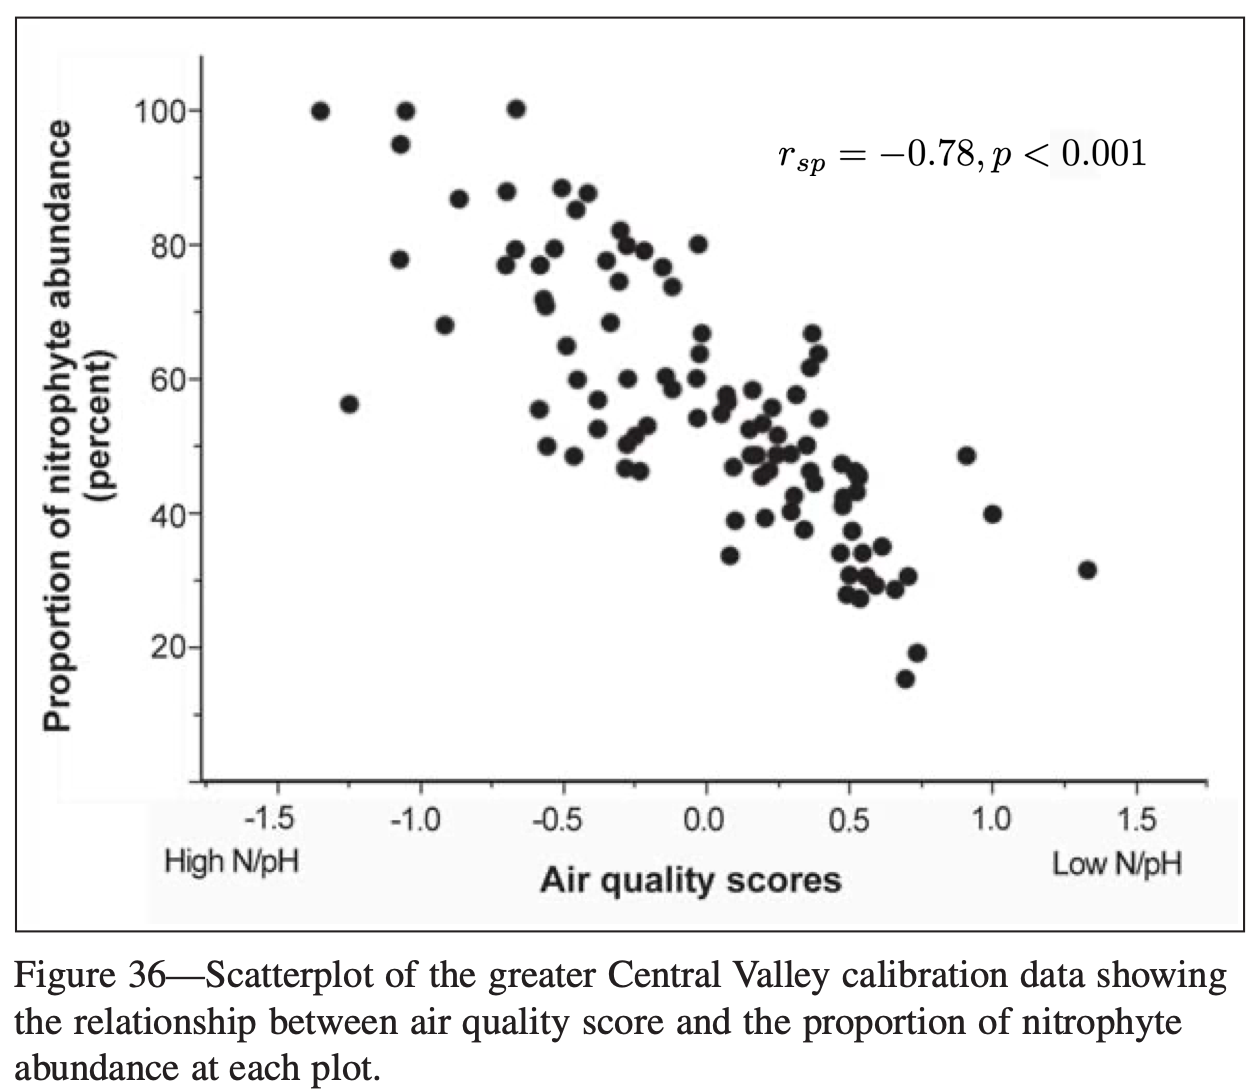
\includegraphics[width=17.47in]{../figures/lichen_abundance} \end{center}

\hfill\break
We note that the relationship between air quality score and proportion
of nitrophyte abundance is plausibly linear.\\
\strut \\

There is a strong negative correlation
(\emph{r}\textsubscript{sp}=-0.78, \emph{p}\textless0.001) between air
quality score and proportion of nitrophyte lichen. This suggests that
this proportion can be used as a bioindicator of air quality.\\

\hfill\break
A Spearman's rank correlation coefficient was calculated in this case
rather than a Pearson correlation coefficient, despite the fact that
both the \emph{x} and \emph{y} variables are plausibly drawn from
normally distributed populations of values, according to a Shapiro-Wilk
test. The problem is that both the air quality score and the proportion
of nitrophyte abundance are ordinal variables - something we learn from
reading the paper in which this figure appears. This means that analysis
using parametric tests such as the Pearson method for determining linear
correlation are not appropriate. A non-parametric method such as
Spearman's rank method can be used instead.\\

\subsubsection{Soil bacteria}\label{soil-bacteria}

Lauber, C. L., Hamady, M., Knight, R., \& Fierer, N. (2009).
Pyrosequencing-based assessment of soil pH as a predictor of soil
bacterial community structure at the continental scale. Applied and
Environmental Microbiology, 75(15), 5111--5120.
\url{https://doi.org/10.1128/AEM.00335-09}

\begin{center}\includegraphics[width=18in]{../figures/soil_bacteria} \end{center}

In the Figure above, note that the Pearson \emph{r}-values for
\textbf{C} and \textbf{E} are close to zero, and the \emph{p}-values are
greater than 0.1, meaning that at this significance level there is no
evidence from these data that there is \emph{any} linear association
between soil pH and the relative abundances of
\emph{Alphaproteobacteria} or \emph{Beta/Gammaproteobacteria}. From the
plots, it looks in \textbf{C} as if there no assocation at all, whereas
in \textbf{E} it looks as though there might be, but if so then not a
linear or even monotonic association, for which the correlation
coefficient r (Pearson or Spearman) would be a poor measure.

\subsection{Exercise 1}\label{exercise-1}

\begin{center}\includegraphics{Correlation_files/figure-latex/unnamed-chunk-36-1} \end{center}

Plots A to F above show scatter plots of different data sets \emph{Y}
against \emph{X}.

\begin{itemize}
\tightlist
\item
  Which of them show linear behaviour?
\item
  Which of them show monotonic behaviour?
\item
  For which of them might it be appropriate to calculate the following
  correlation coefficients between \emph{X} and \emph{Y}?

  \begin{itemize}
  \tightlist
  \item
    Pearson \emph{r}
  \item
    Spearman rank \emph{r}\textsubscript{sp}
  \end{itemize}
\end{itemize}

\subsection{Exercise 2}\label{exercise-2}

Measurements were made on female Adelie penguins on a series of islands
in the Antarctic. The bill lengths and depths of 73 individuals were
recorded and are shown in the plot below.

\begin{center}\includegraphics{Correlation_files/figure-latex/unnamed-chunk-38-1} \end{center}

From this information and plot, decide

\begin{itemize}
\tightlist
\item
  Whether it is plausible that there is a linear relationship between
  the bill depths and lengths within the data set
\item
  Whether the correlation coefficient within the data set is likely to
  be positive or negative
\item
  Whether the correlation is `strong' or `weak' ie is the absolute value
  of the correlation coefficient likely to be close to 1 or close to
  zero
\item
  Whether there might be evidence from this data that there is any
  correlation between bill depth and bill length in the population from
  which this data set was drawn.
\end{itemize}

\paragraph{Tests for normality}\label{tests-for-normality}

Shapiro-Wilk tests are carried out to check for normality of the two
sets of data:

\begin{Shaded}
\begin{Highlighting}[]
\FunctionTok{shapiro.test}\NormalTok{(bill\_depths)}
\end{Highlighting}
\end{Shaded}

\begin{verbatim}
## 
##  Shapiro-Wilk normality test
## 
## data:  bill_depths
## W = 0.9831, p-value = 0.4364
\end{verbatim}

\begin{Shaded}
\begin{Highlighting}[]
\FunctionTok{shapiro.test}\NormalTok{(bill\_lengths)}
\end{Highlighting}
\end{Shaded}

\begin{verbatim}
## 
##  Shapiro-Wilk normality test
## 
## data:  bill_lengths
## W = 0.99117, p-value = 0.8952
\end{verbatim}

On this basis, we see that we can use the Pearson method to calculate
the correlation coefficient between bill depth and bill length. What is
telling us this?

\paragraph{Calculate correlation
coefficient}\label{calculate-correlation-coefficient}

For these data, we calculate the correlation coefficient using the
Pearson method.

\begin{Shaded}
\begin{Highlighting}[]
\CommentTok{\# Pearson}
\FunctionTok{cor.test}\NormalTok{(bill\_depths,bill\_lengths, }\AttributeTok{method =} \StringTok{"pearson"}\NormalTok{)}
\end{Highlighting}
\end{Shaded}

\begin{verbatim}
## 
##  Pearson's product-moment correlation
## 
## data:  bill_depths and bill_lengths
## t = 1.3714, df = 71, p-value = 0.1746
## alternative hypothesis: true correlation is not equal to 0
## 95 percent confidence interval:
##  -0.07209557  0.37677877
## sample estimates:
##       cor 
## 0.1606361
\end{verbatim}

Which part(s) of this output tell us that:

\begin{itemize}
\tightlist
\item
  There is a weak positive correlation between bill length and depth
  \emph{within the sample}?
\item
  There is no evidence that this correlation exists in the wider
  population from which this data set was drawn?
\end{itemize}

How would you report this result?

\subsection{Exercise 3}\label{exercise-3}

Open a new R notebook

In the usual way, include to start with code chunks to

\begin{enumerate}
\def\labelenumi{\arabic{enumi}.}
\tightlist
\item
  Load the packages needed \texttt{tidyverse} and \texttt{here}.
\item
  Read the data set \texttt{iris.csv} (which should be in your data
  folder already) into an object called \texttt{iris}
\end{enumerate}

You can do this with this code chunk:

\begin{verbatim}
```{r}     
filepath<-here("data","iris.csv")
iris<-read_csv(filepath)
glimpse(iris)
```
\end{verbatim}

\begin{enumerate}
\def\labelenumi{\arabic{enumi}.}
\setcounter{enumi}{3}
\item
  Create a faceted plot of sepal length against sepal width for each
  species.
\item
  Calculate the Pearson correlation coefficient between sepal length and
  sepal width for each species, and display this, plus the lower and
  upper bounds of the confidence interval and the \emph{p}-value for
  each species in a table.
\end{enumerate}

For (4) and (5) you can adapt code used on the main Correlation tab.

Now:

\begin{itemize}
\tightlist
\item
  Does it appear that the sepal length and sepal width are correlated
  for each species?\\
\item
  Is the correlation positive or negative?\\
\item
  For which species is the correlation strongest?\\
\item
  Do the correlation coefficients make sense, given the plots?
\end{itemize}

\end{document}
